\documentclass[12pt]{article}
\usepackage[pdfborder={0 0 0.5 [3 2]}, plainpages=false]{hyperref}%
\usepackage[left=1in,right=1in,top=1in,bottom=1in]{geometry}%
\usepackage[shortalphabetic]{amsrefs}%
\usepackage{amsmath}
\usepackage{enumerate}
% \usepackage{enumitem}
\usepackage{amssymb}                
\usepackage{amsmath}                
\usepackage{amsfonts}
\usepackage{amsthm}
\usepackage{bbm}
\usepackage[table,xcdraw]{xcolor}
\usepackage{tikz}
\usepackage{float}
\usepackage{booktabs}
\usepackage{svg}
\usepackage{mathtools}
\usepackage{cool}
\usepackage{url}
\usepackage{graphicx,epsfig}
\usepackage{makecell}
\usepackage{array}

\def\noi{\noindent}
\def\T{{\mathbb T}}
\def\R{{\mathbb R}}
\def\N{{\mathbb N}}
\def\C{{\mathbb C}}
\def\Z{{\mathbb Z}}
\def\P{{\mathbb P}}
\def\E{{\mathbb E}}
\def\Q{\mathbb{Q}}
\def\ind{{\mathbb I}}

\DeclareMathOperator{\spn}{span}
\DeclareMathOperator{\ran}{range}

\graphicspath{ {suspension/} }

\newtheorem{lemma}{Lemma}
\newtheorem{theorem}{Theorem}
\newtheorem{corollary}{Corollary}
\newtheorem{definition}{Definition}
\newtheorem{proposition}{Proposition}
\newtheorem{assumption}{Assumption}
\newtheorem{hypothesis}{Hypothesis}

\newtheorem{notation}{Notation}

\begin{document}

\section{Chen-McKenna Suspension Bridge Equation}

\subsection{Background}

In \cite{McKenna1990}, McKenna and Walter propose the following equation to model traveling waves on an infinitely long suspended beam

\begin{equation}\label{susp}
u_{tt} + u_{xxxx} + u^+ - 1 = 0
\end{equation}

where $u^+ = \max(u, 0)$. In \cite{Chen1997}, Chen and McKenna propose the model

\begin{equation}\label{susp2}
u_{tt} + u_{xxxx} + e^{u} - 1 = 0
\end{equation}

which is a smooth approximation to \eqref{susp}. Making the change of variables $u - 1 \mapsto u$ so that localized solutions will decay to a baseline of 0 instead of 1, we will consider the equation

\begin{equation}\label{susp3}
u_{tt} + u_{xxxx} + e^{u} - 1 = 0
\end{equation}

In a co-moving frame with speed $c$, this becomes

\begin{equation}\label{suspc}
u_{tt} - 2 c u_{x t} + u_{xxxx} + c^2 u_{xx} + e^{u} - 1 = 0
\end{equation}

An equilibrium solution satisfies the ODE

\begin{equation}\label{eqODE}
u_{xxxx} + c^2 u_{xx} + e^{u} - 1 = 0
\end{equation}

In \cite{Smets2002} (Theorem 11), Smets and van den Berg prove existence of a localized, symmetric traveling wave solution $q(x; c)$ to \eqref{susp2} for almost all speeds $c \in (0, \sqrt{2})$. In \cite{Berg2018}, van den Berg et al use a computer-assisted proof technique (Theorem 1) to prove existence of such solutions to \eqref{susp2} for all speeds $c$ with $c^2 \in [0.5, 1.9]$.\\

We are interested in the existence and stability of multi-pulse solutions to \eqref{suspc}. First, we look at existence. For any solution $u_*$ to \eqref{eqODE}, the linearization of \eqref{eqODE} about $u_*$ is given by

\begin{equation}\label{defA0}
A_0(u^*) = \partial_x^4 + c^2 \partial_x^2 + e^{u_*}
\end{equation}

For $c \in (0, \sqrt{2})$, $A_0(0)$ is hyperbolic, and its spectrum is given by

\begin{align}\label{specA00}
\sigma(A_0(0)) &= \pm \alpha \pm \beta i && \alpha, \beta > 0
\end{align}

In addition, equation \eqref{eqODE} is Hamiltonian with energy

\begin{equation}\label{defH}
H(u) = u_x u_{xxx} - \frac{1}{2}u_{xx}^2 + \frac{c^2}{2}u_x^2 + e^u - u
\end{equation}

We also make the following hypothesis.

\begin{hypothesis}\label{A0kernel}
The operator $A_0(q(x; c))$ has a one-dimensional kernel spanned by $\partial_x q(x; c)$.
\end{hypothesis}

from which it follows that the primary pulse $q(x; c)$ is transversely constructed. Thus we have the following theorem, which is adapted from Theorem 3.6 in \cite{Sandstede1997}.

\begin{theorem}\label{multiexist}
Let $q(x; c)$ be a localized solution to \eqref{eqODE} such that Hypothesis \ref{A0kernel} holds. Then for any $n \geq 2$ and any sequence of nonnegative integers $k_0, \dots, k_{n-1}$ with at least one of the $k_j \in \{0, 1 \}$, there exists a nonnegative integer $m_0$ such that
\begin{enumerate}
	\item For any nonnegative integer $m$ with $m \geq m_0$, there exists a unique $n-$modal solution $q_n(x, c)$ to \eqref{eqODE} which is of the form
	\begin{align}\label{qn}
	q_n(x; c) = \sum_{j = 1}^{n} q^j(x; c) + r(x; c)
	\end{align}
	where each $q^j(x; c)$ is a translate of the primary pulse $q(x; c)$. The distance between the peaks of $q^j$ and $q^{j+1}$ is $2 X_j$, where
	\begin{equation}
	X_j \approx \frac{\pi}{\beta}(2 m + k_j) + \tilde{X}
	\end{equation}
	and $\tilde{X}$ is a constant. The remainder term $r(x; c)$ has uniform bound
	\begin{equation}\label{rbound}
	||r|| \leq C e^{-\alpha X_m}
	\end{equation}
	where $X_m = \min\{X_1, \dots, X_{n-1}\}$.
	\item The linear operator $A_0(q_n)$ has precisely $n$ real eigenvalues $\nu_j$ near 0, where $\nu_1 = 0$ is a simple eigenvalue and $\nu_j = \mathcal{O}(e^{-2\alpha X_m})$ for $j = 2, \dots, n$. Moreover, for $j = 2, \dots, n$,
	\begin{align*}
	\nu_j < 0 \text{ if } k_j \text{ is odd} \\
	\nu_j > 0 \text{ if } k_j \text{ is even} 
	\end{align*}
\end{enumerate}

\begin{proof}
Using \eqref{specA00}, \eqref{defH}, and Hypothesis \ref{A0kernel}, this follows from Theorem 3.6 in \cite{Sandstede1997}. The bound on $r(x; c)$ in (i) follows from \cite{Sanstede1993} and \cite{Sandstede1998}. The eigenvalues $\nu_j$ are real since $A_0(q_n)$ is self-adjoint. The signs of the eigenvalues in (iii) follow from \cite{Sandstede1997} and the fact that the Melnikov integral $M = \int_{-\infty}^\infty |q_x|^2 dx > 0$.
\end{proof}
\end{theorem}

To determine linear stability of these multi-pulse solutions, we look at the linearization of the PDE \eqref{suspc} about $q_n(x; c)$, which is the following quadratic eigenvalue probem

\begin{equation}\label{quadeig}
P_2(\lambda; q_n)v =  [A_2 \lambda^2 + A_1 \lambda + A_0(q_n)]v = 0
\end{equation}

where $A_0(q_n)$ is defined in \eqref{defA0} and 

\begin{align}
A_1 &= -2 c \partial_x \\
A_2 &= I
\end{align}

We will use the Krein matrix to find the eigenvalues of \eqref{quadeig}. Applying Theorem \ref{multiexist}, let $\nu_1, \dots, \nu_n$ be the small eigenvalues of $A_0(q_n)$, and let $s_1, \dots, s_n$ be the corresponding eigenfunctions. Define the space $S$ by

\begin{equation}\label{defS}
S = \spn\{s_1, \dots, s_n \}
\end{equation}

and define the Krein matrix $K_S(z)$ as on p.4 of Kap2018. We make the following hypotheses.

\begin{hypothesis}\label{PDEexisthyp}
For every initial condition $u_0(x)$ there exists a solution $u(x, t)$ to \eqref{suspc} on the interval $I = [0, T]$, where $T$ only depends on $\max{ \{ ||u_0||, ||(u_0)_t|| \} }$.
\end{hypothesis}

\begin{hypothesis}\label{A0neg}
The operator $A_0(q)$ has a unique, simple negative eigenvalue $\lambda_- < 0$ with corresponding eigenfunction $v_-(x)$.
\end{hypothesis}

\begin{hypothesis}\label{dccpos}
$d''(c) > 0$ for $c^2 \in (0, 2)$, where $d(c)$ is defined in (2.16) of \cite{Grillakis1987} and 

\begin{equation}\label{dcc}
d''(c) = -\frac{\partial}{\partial c} \left( c ||q_x||^2 \right)
\end{equation}
\end{hypothesis}

We now present the following theorem, which is the main result of this section.

\begin{theorem}\label{Kreindiag}
Let $q_n(x; c)$ be an $n-$modal solution to \eqref{eqODE}. Assume Hypotheses \ref{A0kernel}, \ref{existhyp}, \ref{A0neg}, and \ref{dccpos}. Then the Krein matrix is given by

\begin{equation}\label{Kreinapprox}
K_S(z) = ||q_x||^2 \text{diag} (\nu_1, \dots, \nu_n)
 + d''(c) I \overline{z}^2 + \mathcal{O}(e^{-(3 \alpha/2) X_m}|z| + |z|^3)
\end{equation}

which is diagonal to leading order.

\end{theorem}

As a corollary, we have the following criteria for linear stability and instability of the multi-pulse solutions $q_n(x; c)$.

\begin{corollary}\label{stabcrit}
Let $q_n(x; c)$ be an $n-$pulse solution to \eqref{eqODE}, and assume the same hypotheses as in Theorem \ref{Kreindiag}. Let $\nu_1, \dots, \nu_n$ be the small eigenvalues of $A_0(q_n)$, as defined in Theorem \ref{multiexist}, where $\nu_1 = 0$.
\begin{enumerate}
	\item If $\nu_2, \dots, \nu_n < 0$, then \eqref{quadeig} has $2n$ purely imaginary eigenvalues near 0, which are given by

	\begin{equation}\label{npulseKreineigs}
	\lambda_j^\pm = \pm i \left( ||q_x|| \sqrt{ \frac{|\nu_j|}{d''(c)} } + \mathcal{O}(e^{-(3 \alpha/2) X_m}) \right)
	\end{equation}

	Thus $q_n(x; c)$ is linearly neutrally stable.

	\item If $\nu_j > 0$ for some $j = 2, \dots, n$, then \eqref{quadeig} has at least one eigenvalue with positive real part. Thus $q_n(x; c)$ is linearly unstable.
\end{enumerate}

\end{corollary}

\subsection{Numerics}

This primary pulse solution $q(x; c)$ can be constructed numerically using the string method in \cite{Chamard2011}. The following figure shows these solutions for the same values of $c$ as in Figure 3 of \cite{Chen1997}.

\begin{figure}[H]
\centering
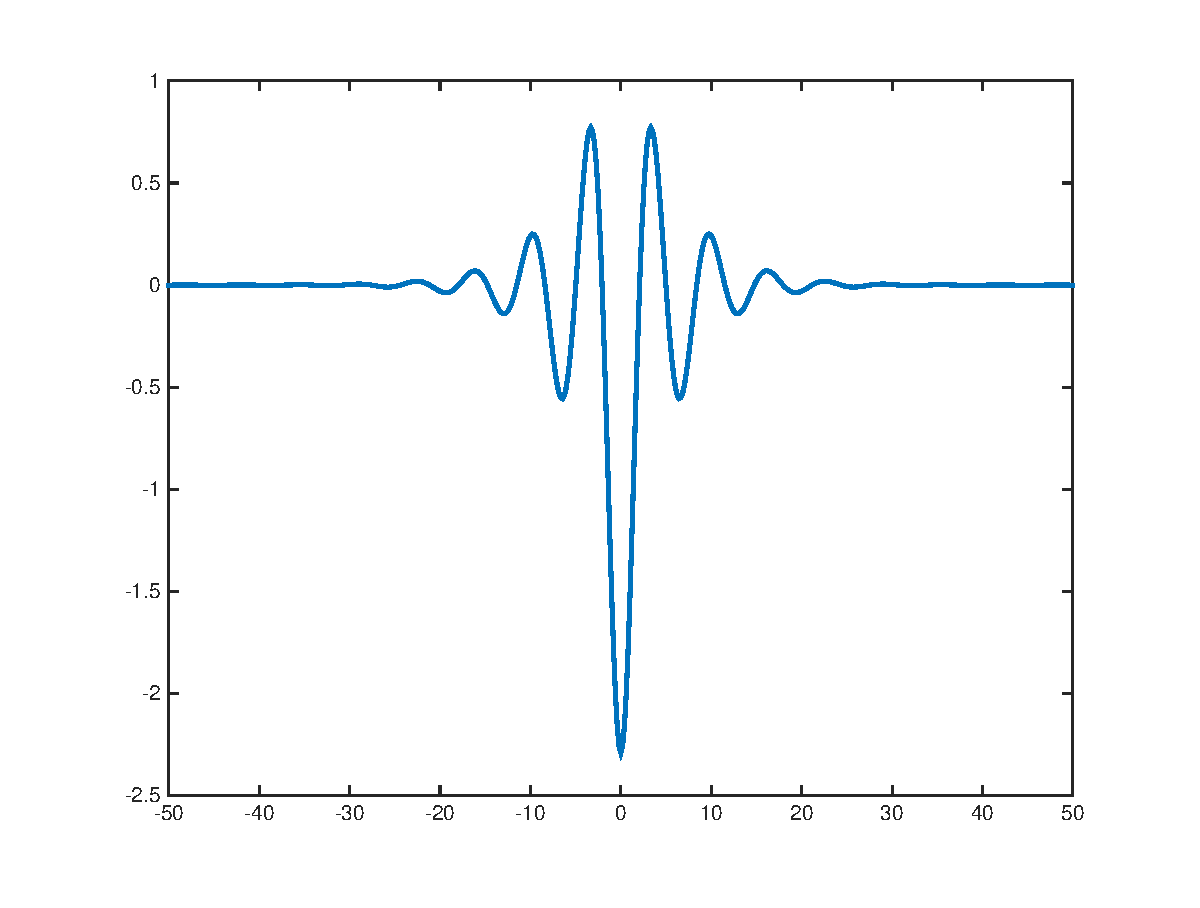
\includegraphics[width=8cm]{single1354.eps}
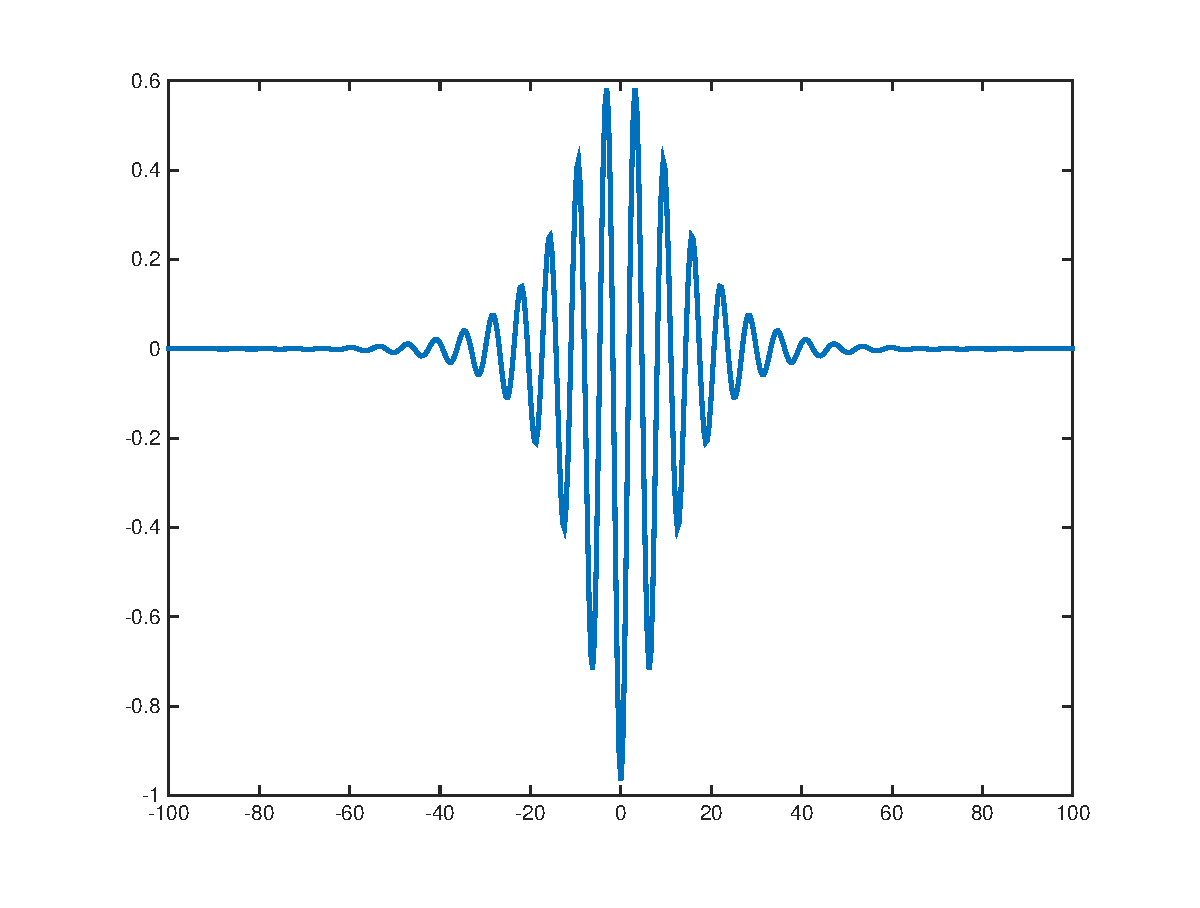
\includegraphics[width=8cm]{single14.eps}
\label{fig:single1}
\caption{Primary pulse solutions $q(x;c)$ to \eqref{eqODE} for $c = 1.354$ (left) and $c = 1.40$ (right). Finite difference methods, $N = 512$.}
\end{figure}

\subsection{Eigenvalue Problem}

For linear stability analysis, we look at the PDE eigenvalue problem. Let $u_*(x)$ be an exponentially localized equilibrium solution of \eqref{eqODE}. We use the standard linearization ansatz

\begin{equation}
u(x,t) = u_*(x) + \epsilon e^{\lambda t} v(x)
\end{equation}

and keep only terms of order $\epsilon$ to obtain the quadratic eigenvalue problem

\begin{equation}\label{quadeig}
P_2(\lambda; u_*)v =  [A_2 \lambda^2 + A_1 \lambda + A_0(u_*)]v = 0
\end{equation}

where

\begin{align}
A_0(u^*) &= \partial_x^4 + c^2 \partial_x^2 + e^{u_*} \\
A_1 &= -2 c \partial_x \\
A_2 &= I
\end{align}

We note that if $\lambda$ is an eigenvalue, so is $\overline{\lambda}$, and if $u_*(x)$ is an even function, $-\lambda$ is also an eigenvalue. Thus is we linearize about an even function, we have the typical four-fold symmetry of eigenvalues.\\

For $c \in (0, \sqrt{2})$, by the Weyl essential spectrum theorem, the essential spectrum of \eqref{quadeig} is independent of $u_*$ and is given by

\begin{equation}\label{ess}
\sigma_{\text{ess}}(P_2) = (-\infty, \rho] \cup [\rho, \infty)
\end{equation}

where $\rho > 0$ and is the minimum of the function $\lambda(r) = c r + \sqrt{1 + r^4}$; this minimum is positive for $c \in (0, \sqrt{2})$. Thus the essential spectrum is bounded away from 0.\\

The linear operator $A_0(u_*)$ is the linearization of \eqref{eqODE} about $u_*$. We note that $\partial_x u_*$ is an eigenfunction of $A_0(u_*)$ with eigenvalue 0. By the Weyl essential spectrum theorem, the essential spectrum of $A_0(u^*)$ is independent of $u_*$ and is given by

\begin{equation}\label{A0ess}
\sigma_{\text{ess}}(A_0(u_*)) = [1 - c^4/4, \infty)
\end{equation}

which is positive and bounded away from 0 for $c \in (0, \sqrt{2})$. If we linearize about a single pulse solution $q(x; c)$ and compute the spectrum numerically using Matlab's \texttt{eig} function, we note the presence of a simple negative eigenvalue, as well as the eigenvalue at 0 and the essential spectrum \eqref{A0ess}.

\begin{figure}[H]
\centering
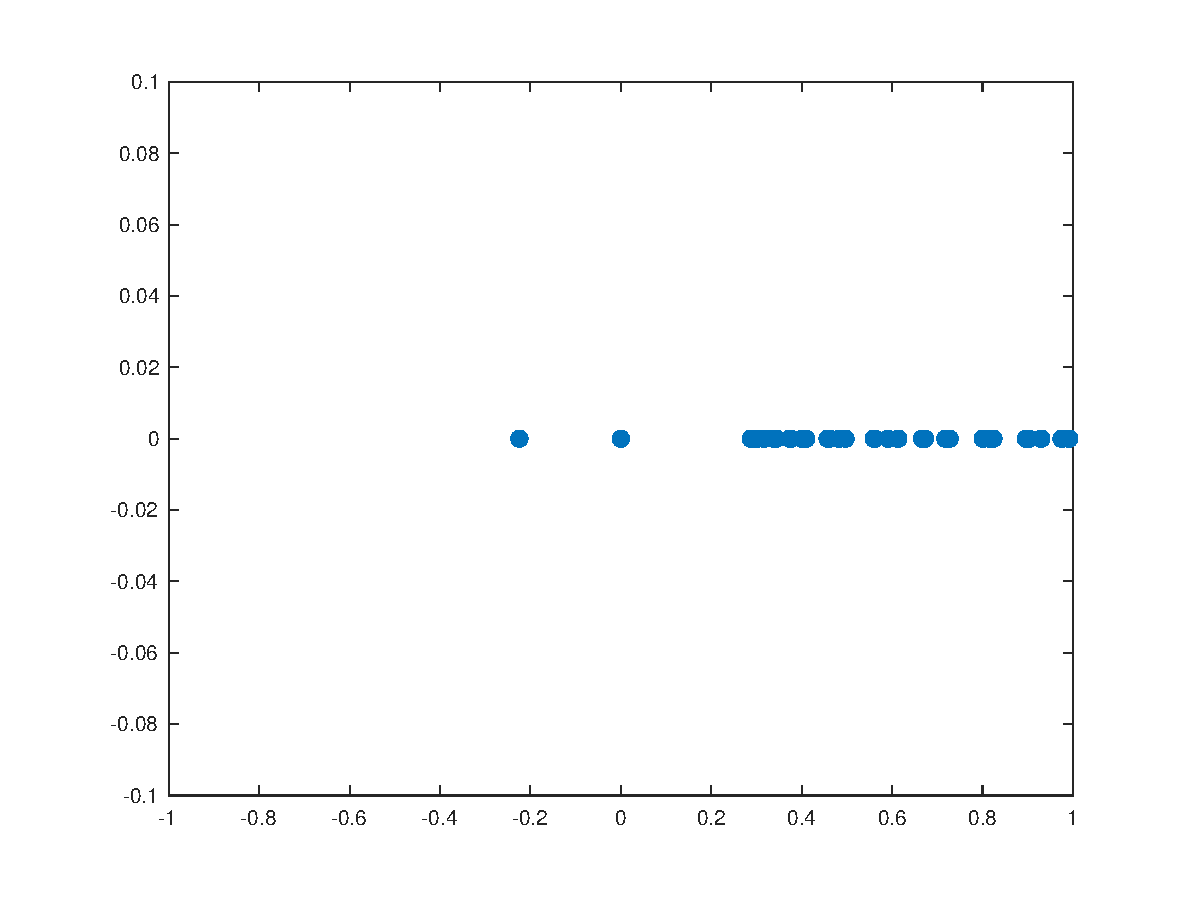
\includegraphics[width=8cm]{specA0.eps}
\caption{Spectrum of $A_0(q)$, the linearization about a single pulse $q$. $c = 1.3$. Finite difference methods, $N = 513$.}
\end{figure}

Based on this numerical result, we make the following hypothesis.

\begin{hypothesis}\label{hyp_A0neg}
\begin{enumerate}[(i)]
\mbox{}
\item For any exponentially localized equilibrium solution $u_*(x)$ to \eqref{eqODE}, the operator $A_0(u_*)$ has a one-dimensional kernel spanned by $\partial_x u_*(x)$. 
\item For a single-pulse solution $q(x; c)$ to \eqref{eqODE}, the operator $A_0(q)$ has exactly one negative eigenvalue $\lambda_- < 0$ with corresponding eigenfunction $v_-(x)$.
\end{enumerate}
\end{hypothesis}

We also note that 

\begin{equation}\label{uc}
A_0(u_*) \partial_c u^* = -2 c u^*_{xx}
\end{equation}

\subsection{Stability of the Primary Pulse}

Letting $v = u_t$, we can write \eqref{susp3} as the Hamiltonian system

\begin{equation}\label{2dsystem}
\frac{d \textbf{u} }{dt} = J E'(\textbf{u})
\end{equation}

where $\textbf{u} = \begin{pmatrix}u&v\end{pmatrix}^T$, $J$ is the standard symplectic matrix

\begin{equation*}
J = \begin{pmatrix}0 & 1 \\ -1 & 0 \end{pmatrix}
\end{equation*}

and $E(\textbf{u})$ is the energy

\begin{equation}\label{energy}
E(\textbf{u}) = \int_{-\infty}^\infty \left(\frac{1}{2} v^2 + \frac{1}{2}u_{xx}^2 + e^{u} - u \right)dx
\end{equation}

The equation \eqref{2dsystem} and the energy \eqref{energy} are invariant under the unitary translation group $T(s)$, defined by $T(s)\phi(\cdot) = \phi(\cdot - s)$. \\

We make the following hypothesis regarding the existence of solutions to \eqref{2dsystem}.

\begin{hypothesis}\label{existhyp}
For every initial condition $\textbf{u}_0$ there exists a solution $\textbf{u}(t)$ to \eqref{2dsystem} on the interval $I = [0, T]$, where $T$ only depends on $||\textbf{u}_0||$, such that $\textbf{u}(0) = \textbf{u}_0$. 
\end{hypothesis}

Using \cite{Grillakis1987} together with Hypothesis \ref{A0neg} and Hypothesis \ref{existhyp}, we have the following stability criterion for the primary pulse $q(x; c)$. 

\begin{proposition}\label{stabcrit}
Let $c^2 \in [0.5, 1.9]$, and let $q(x; c)$ be the single pulse solution to \eqref{eqODE} associated with this speed $c$. Then $q(x; c)$ is stable if and only if $d''(c) > 0$, where $d(c)$ is defined in (2.16) of \cite{Grillakis1987} and 

\begin{equation}\label{dcc}
d''(c) = -\frac{\partial}{\partial c} \left( c ||q_x||^2 \right)
\end{equation}

\begin{proof}
We need to verify Assumptions 1, 2, and 3B in \cite{Grillakis1987}. Assumption 1 is the same as Hypothesis \ref{existhyp}. Assumption 2 follows from the fact that $q(x; c)$ is a bound state, i.e. satisfies (2.15) in \cite{Grillakis1987}, and from smooth dependence of the solution $q(x; c)$ of \eqref{eqODE} on the parameter $c$. Assumption 3B follows from Hypothesis \ref{A0neg} and the corrected proof of Lemma 6.2 in \cite{Grillakis1987} given in \cite{Grillakis1990}. The result follows from Theorem 5.5 and Theorem 3 in \cite{Grillakis1987}.

\end{proof}
\end{proposition}

For this equation \eqref{suspc}, numerical analysis suggests that $d''(c) > 0$, indicating that $q(x; c)$ is stable. We therefore make the following hypothesis.

\begin{hypothesis}\label{hyp_dccpos}
$d''(c) > 0$ for $c^2 \in [0.5, 1.9]$.
\end{hypothesis}

\subsection{Multipulse Solutions}

Let $q(x; c)$ be the primary pulse solution to \eqref{eqODE}. We make the following hypothesis regarding the primary pulse.

\begin{hypothesis}\label{transverseq}
The primary pulse $q(x; c)$ is transversely constructed, i.e. 
\[
T_{q(0; c)} W^s(0; c) \cap T_{q(0; c)} W^u(0; c) = \R q'(0; c).
\]
\end{hypothesis}

Since \eqref{eqODE} has a hyperbolic equilibrium at 0 and is a Hamiltonian system, we can use Lin's method (\cite{Sanstede1993}, \cite{Sandstede1997}, \cite{Sandstede1998}) to construct an $n-$pulse solution $q_n$ to \eqref{eqODE}. This solution resembles, to leading order, $n$ copies of the primary pulse $q$ joined together and separated by distances $2 X_1, \dots 2 X_{n-1}$. We can write $q_n$ as 

\begin{align}\label{qn}
q_n = \sum_{i = 1}^{n} q^i + r
\end{align}

where each function $q^i$ is a translate of the primary pulse $q$

\begin{equation}\label{qi}
q^i(\cdot) = q(\cdot - L_i)
\end{equation}

and the remainder term $r$ has uniform bound

\begin{equation}
||r|| \leq C e^{-\alpha X_m}
\end{equation}

where

\begin{equation}\label{defXm}
X_m = \min\{X_1, \dots, X_n \}
\end{equation}

This bound holds for all derivatives with respect to $x$. $X_m$ is sufficiently large that the $n$ peaks are exponentially separated.\\

We can construct these multipulse solutions numerically by joining together the oscillatory tails of the primary pulse. This join can only be performed every quarter period, i.e. every $\pi / 2 \beta$ (\cite{Sandstede1997}). After gluing primary pulses together at the appropriate intervals, the multipulse solution is found numerically using Matlab's \texttt{fsolve} function.The first four double pulse solutions for $c = 1.2$ are shown in Figure \ref{fig:double}.

\begin{figure}[H]
\label{fig:double}
\centering
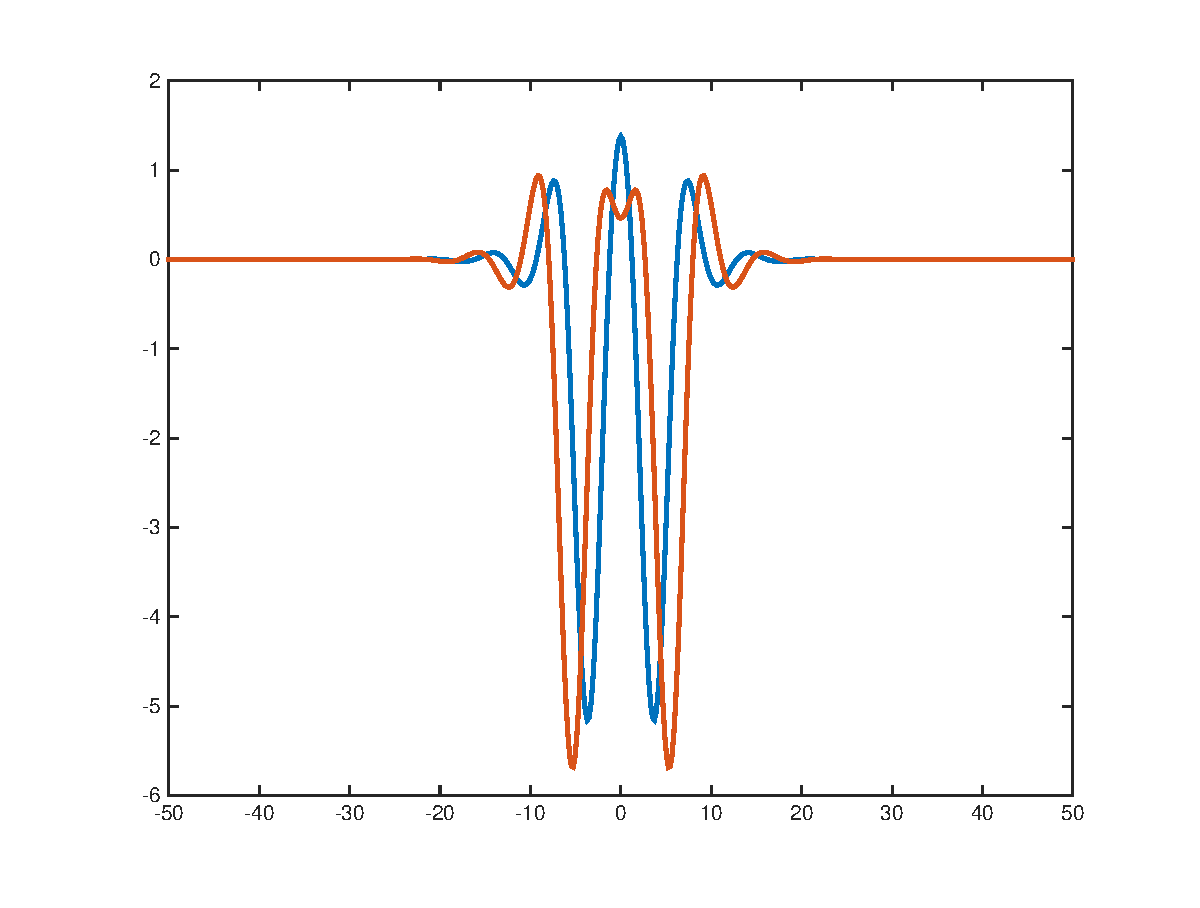
\includegraphics[width=8cm]{double12_12.eps}
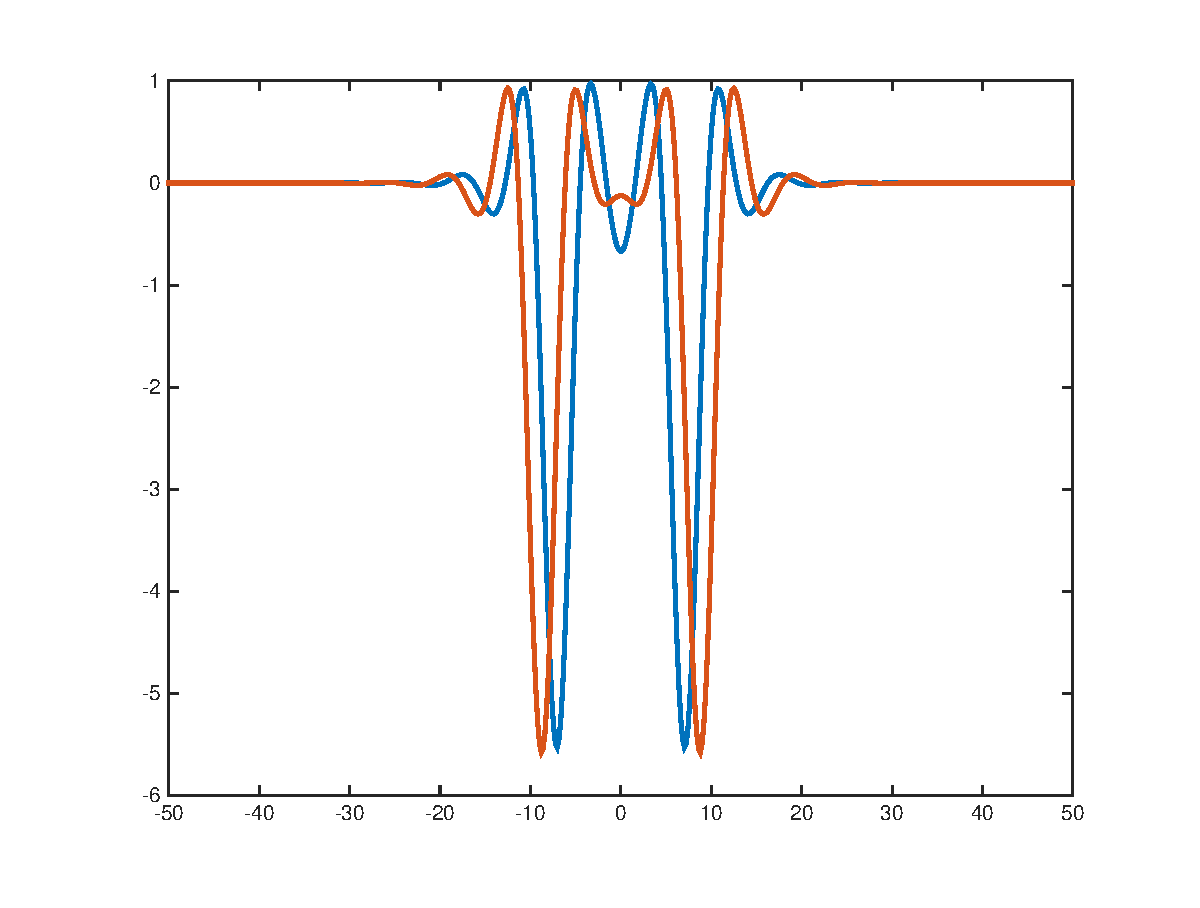
\includegraphics[width=8cm]{double12_34.eps}
\caption{Double pulse solutions $q_2(x; c)$ to \eqref{eqODE} for $c = 1.2$. Double pulses 1 and 2 (left). Double pulses 3 and 4 (right).}
\end{figure}

Using Lin's method again (\cite{Sandstede1998}), the linear operator $A_0(q_n)$ has $n$ distinct small eigenvalues near 0 (by Hypothesis \ref{A0neg}, this includes one eigenvalue at 0 corresponding to the kernel eigenfunction $\partial_x q_n$). Let $\{\nu_1, \dots, \nu_n\}$ be these small eigenvalues (chosen so that $\nu_1 = 0$), and let $\{s_1, \dots, s_n \}$ be the corresponding eigenfunctions. From Lin's method (\cite{Sandstede1998}, we have

\begin{equation}
|\nu_i| = \mathcal{O}(e^{-2 \alpha X_m})
\end{equation}

Since $A_0(q_n)$ is self-adjoint and the eigenvalues $\nu_i$ are distinct, the eigenfunctions $s_i$ are orthogonal. We scale the eigenfunctions $s_i$ so that

\begin{equation}\label{orthonormaleigs}
\langle s_i, s_j \rangle = ||q_x(x; c)||^2 \delta_{ij}
\end{equation}

From \cite{Sandstede1998}, the eigenfunctions $s_i$ are, to leading order, linear combinations of translates of the derivative of the primary pulse. In other words, for $j = 1, \dots, n$

\begin{align}\label{sj}
s_j = \sum_{i = 1}^{n} d_{ji} q^i_x + w_j
\end{align}

for constants $d_{ji} \in \C$, where the $q^i$ are defined in \eqref{qi}. The remainder terms $w_j$ have a uniform bound

\begin{equation}\label{sjwbound}
||w_j|| \leq C e^{-2 \alpha X_m}
\end{equation}

which also holds for derivatives with respect to $x$.\\

We can find these eigenvalues numerically as well. The eigenvalues of $A_0(q_2)$ for the first two double pulses are shown in Figure \ref{fig:specA0double}.

\begin{figure}[H]
\label{fig:specA0double}
\centering
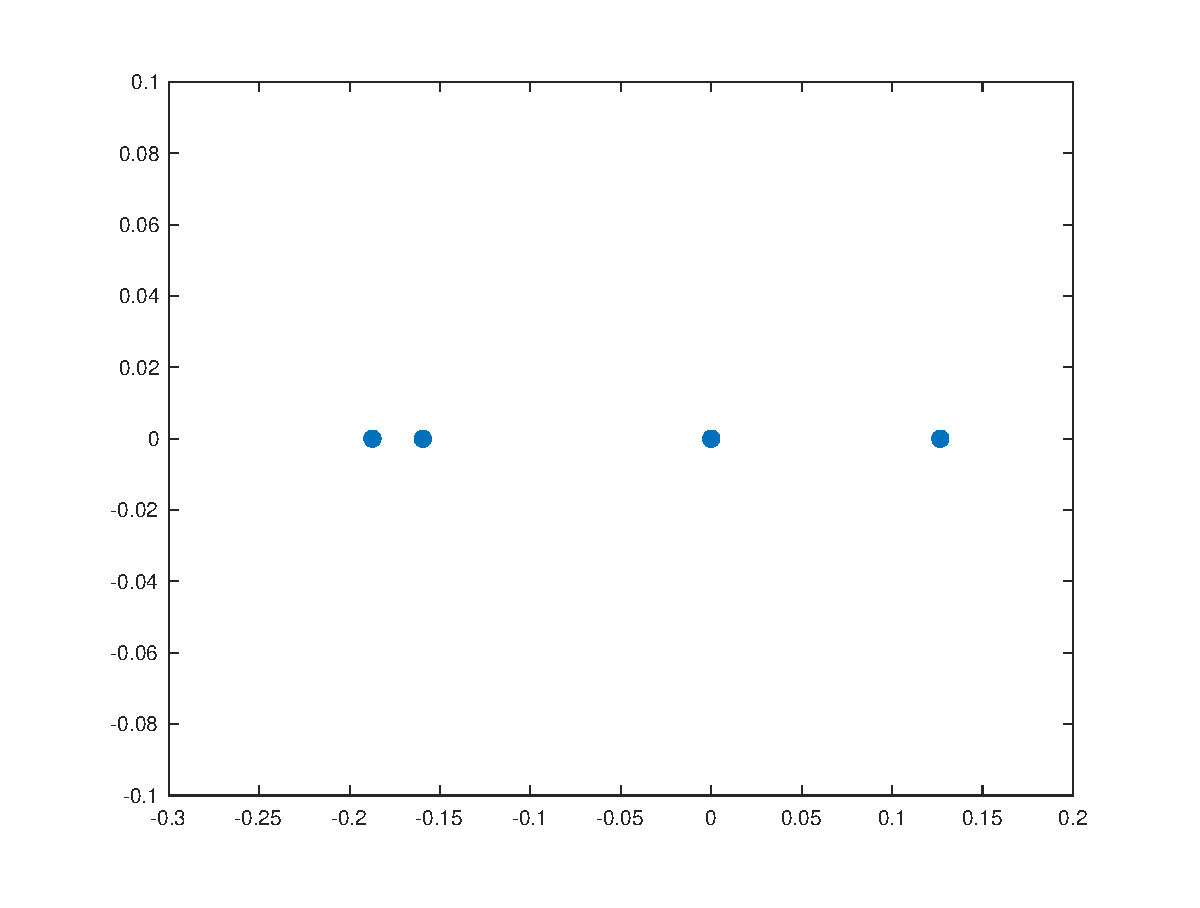
\includegraphics[width=8cm]{specA0d1}
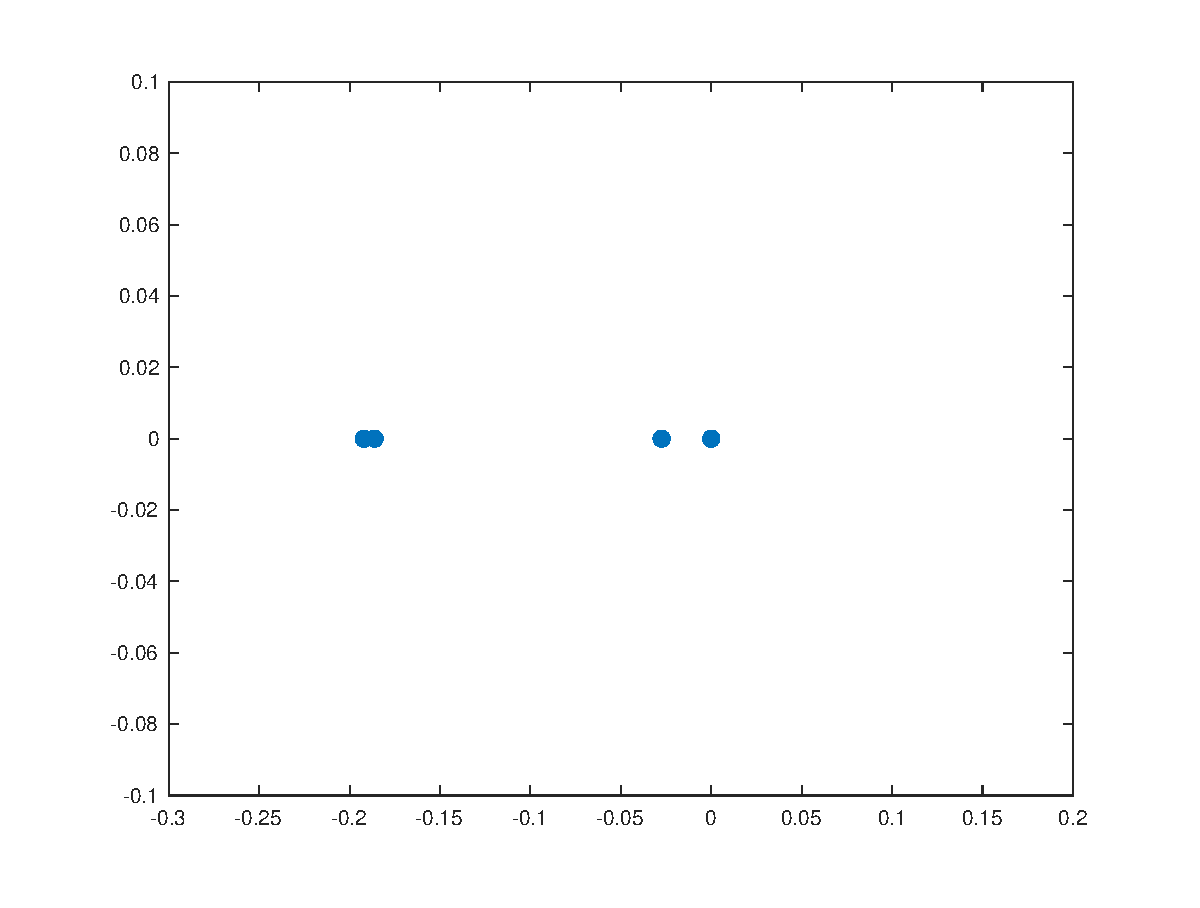
\includegraphics[width=8cm]{specA0d2}
\caption{Eigenvalues of $A_0(q_2)$ for $c = 1.2$. Double pulses 1 (left) and double pulses 2 (right).}
\end{figure}

Note that there are two small eigenvalues near 0 and a clump of two negative eigenvalues, i.e. the eigenvalues for $A(q)$ have each split into a pair. For double pulse 1, the small eigenvalue near 0 is positive, whereas for double pulse 2, this eigenvalue is negative. This pattern of alternating positive and negative eigenvalues continues as the peak distance is increased.

\subsection{Krein Matrix}

We can now use the Krein matrix to compute eigenvalues of \eqref{quadeig}, the linearization of \eqref{suspc} about a multipulse solution $q_n(x; c)$. Let $S$ be the subspace spanned by the eigenfunctions of $A_0(q_n)$ corresponding to the $n$ eigenvalues near 0.

\begin{equation}\label{defS}
S = \spn\{s_1, \dots, s_n \}
\end{equation}

We use the approximation in Section 5 (of Kap2018). Let $\lambda = i z$. Using Lemma 5.6, for small $|z|$ the Krein matrix is the $n \times n$ matrix

\begin{equation}\label{Kreinform}
K_S(z) = ||q_x||^2 \text{diag}(\nu_1, \dots, \nu_n) + \overline{z} K_1 
- \overline{z}^2 ( ||q_x||^2 I + K_2) + \mathcal{O}(|z|^3)
\end{equation}

where

\begin{align}
(K_1)_{jk} &= \langle s_j, i A_1 s_k \rangle \\
(K_2)_{jk} &= \langle P_{S^\perp} A_1 s_j, (P_{S^\perp} A_0(q_n)|_{S^\perp})^{-1} P_{S^\perp} A_1 s_k \rangle
\end{align}

Compared to Lemma 5.6, we have omitted the $-z$ out front, i.e. we use the form of the Krein matrix from p.4. We have also scaled the eigenfunctions differently, which accounts for the additional factor of $||q_x||^2$ in the first term. This is, to leading order, a matrix-valued quadratic polynomial in $z$ (and its complex conjugate). If we take $z$ to be real, the Krein matrix is Hermitian.\\

First, we characterize the Krein matrix for the 1-pulse, since in that case it will be a scalar.

% Lemma : Krein matrix, 1-pulse

\begin{lemma}\label{Krein1pulse}
For the linearization about the 1-pulse, the Krein matrix is the scalar

\begin{equation}
K(z) = d''(c) \overline{z}^2 + \mathcal{O}(z^3)
\end{equation}

where $d''(c)$ is given in \eqref{dcc} and is the stability criterion from \cite{Grillakis1987}.

\begin{proof}
For the 1-pulse $q$, there is exactly one eigenvalue at 0, for which the corresponding eigenfunction is $q_x$. Let $S = \ker A_0(q)$ = $\spn \{q_x\}$. Since $K_1 = 0$, the Krein matrix reduces to the scalar

\begin{align*}
K(z) &= -\overline{z}^2 \left( ||q_x||^2 + 4 c^2 \langle P_{S^\perp} q_{xx}, (P_{S^\perp} A_0(q_n)|_{S^\perp})^{-1} P_{S^\perp} q_{xx} \rangle \right) + \mathcal{O}(z^3)
\end{align*}

Since $S$ is the span of a single odd function and $q_{xx}$ is an even function, $P_{S^\perp} q_{xx} = q_{xx}$. Using \eqref{uc} and integrating by parts, the Krein matrix becomes

\begin{align*}
K(z) &= -\overline{z}^2 \left( \langle q_x, q_x \rangle - 2c \langle q_{xx}, q_c \rangle \right) + \mathcal{O}(z^3) \\
&= -\overline{z}^2 \left( \langle q_x, q_x \rangle + c \frac{\partial}{\partial c}\langle q_x, q_x \rangle \right) + \mathcal{O}(z^3)  \\
&= -\frac{\partial}{\partial c} \left( c||q_x||^2 \right) \overline{z}^2  + \mathcal{O}(z^3) 
\end{align*}

\end{proof}
\end{lemma}

For the $n-$pulse $q_n$, the Krein matrix is diagonally dominant, as we show in the following theorem.

% theorem : Krein matrix diag dominant

\begin{theorem}\label{Kreindiagdom}
For the linearization of the suspension bridge equation \eqref{susp3} about an $n-$pulse equilibrium solution $q_n(x)$, the Krein matrix is diagonal to leading order and is given by

\begin{equation}\label{Kreinapprox}
K_S(z) = ||q_x||^2 \text{diag} (\nu_1, \dots, \nu_n)
 + d''(c) I \overline{z}^2 + \mathcal{O}(e^{-(3 \alpha/2) X_m}|z| + |z|^3)
\end{equation}

\begin{proof}
For the matrix $K_1$ in \eqref{Kreinform}, $(K_1)_{jk} = 2 c i \langle s_j, (s_k)_x \rangle$. Using the expansion \eqref{sj} for the eigenfunctions $s_i$ of $A_0(q_n)$,

\begin{align}
\langle s_j &, (s_k)_x \rangle 
&= \sum_{i = 1}^{n} d_{ji} d_{ki} \langle q^i_x, q^i_{xx} \rangle 
+ \sum_{i \neq l} d_{ji} d_{kl} \langle q^i_x, q^l_{xx} \rangle 
+ \langle s_j, (w_k)_x \rangle 
+ \sum_{i = 1}^{n} d_{ki} \langle w_j, q^j_{xx} \rangle
\end{align}  

By translation invariance, $\langle q^i_x, q^i_{xx} \rangle = \langle q_x, \partial_x q_x \rangle = 0$ since $\partial_x$ is skew-symmetric. For $i \neq l$, $q^i$ and $q^l$ are exponentially separated by at least $2 X_m$, so $\langle q^i_x, q^l_{xx} \rangle = \mathcal{O}(e^{-(3 \alpha/2) X_m})$. The last two terms are $\mathcal{O}(e^{-2 \alpha X_m})$ using Holder's inequality and the remainder bound \eqref{sjwbound}. Thus 

\begin{equation}\label{K1final}
K_1 = \mathcal{O}(e^{-(3 \alpha/2) X_m})
\end{equation}

For the matrix $K_2$, again using the expansions \eqref{sj}, we have

\begin{align}\label{K2expansion}
(K_2)_{jk} 
= 4 c^2 \langle &\sum_{i = 1}^{n} d_{ji} q^i_{xx} + (w_j)_x, \\
&\sum_{i = 1}^{n} d_{ki} P_{S^\perp} (P_{S^\perp} A_0(q_n)|_{S^\perp})^{-1} P_{S^\perp} q^i_{xx} + P_{S^\perp} (P_{S^\perp} A_0(q_n)|_{S^\perp})^{-1} P_{S^\perp} (w_k)_x \rangle \nonumber 
\end{align}

The operator $P_{S^\perp} A_0(q_n)$ is self-adjoint and is Fredholm with index 0, thus the restriction $P_{S^\perp} A_0(q_n)|_{S^\perp}$ is invertible on $S^\perp$. The spectrum of $P_{S^\perp} A_0(q_n)|_{S^\perp}$ is bounded away from 0, thus by the resolvent bound for normal operators, $(P_{S^\perp} A_0(q_n)|_{S^\perp})^{-1}$ is a bounded linear operator on $S^\perp$. \\

To evaluate $(P_{S^\perp} A_0(q_n)|_{S^\perp})^{-1} P_{S^\perp} q^i_{xx}$, we first note that since $P_{S^\perp} q^i_{xx}$ is smooth, so is $(P_{S^\perp} A_0(q_n)|_{S^\perp})^{-1} P_{S^\perp} q^i_{xx}$. Using Lin's method, we will look for a solution $y$ to 

\begin{equation}\label{Linstart}
(P_{S^\perp} A_0(q_n))y = P_{S^\perp} q^i_{xx}
\end{equation}

of the form 

\begin{equation}\label{Linsolform}
y = -\frac{1}{2c} P_{S^\perp} q^i_c + \tilde{w}
\end{equation}

where this ansatz is suggested by \eqref{uc}. Substituting \eqref{Linsolform} into \eqref{Linstart} and simplifying, we are left with

\begin{equation}
A_0(q_n)\tilde{w} + h(x) = 0
\end{equation}

where $||h(x)|| = \mathcal{O}(e^{-\alpha X_m})$. Since the translates $q^i(x)$ are exponentially separated, for $i = 1, \dots, n$, we can write the operator $A_0(q_n)$ as 

\begin{align}\label{A0expansion} 
A_0(q_n) &= A_0(q^i) + \sum_{j \neq i} (e^{q^j(x)} - 1) + \tilde{h}(x)
\end{align}

where $||\tilde{h}|| = \mathcal{O}(e^{-\alpha X_m})$. Following \cite{Sandstede1998}, we write this as a piecewise first-order system in $n$ pieces, where we use the expansion \eqref{A0expansion} on the $i$th piece. From this, we obtain a piecewise solution 

\begin{equation}\label{Linpiecesol}
y_i^\pm = -\frac{1}{2c} P_{S^\perp} q^i_c + \tilde{w}_i^\pm
\end{equation}

to \eqref{Linstart} where we have uniform bound $||\tilde{w}_i^\pm|| = \mathcal{O}(e^{-2 \alpha X_m})$. In general, this solution will have $n - 1$ jumps. In this case, however, it will be smooth since \eqref{Linstart} has a unique, smooth solution which must be the same as \eqref{Linpiecesol}. Thus we conclude that 

\begin{equation}\label{invqxx}
(P_{S^\perp} A_0(q_n)|_{S^\perp})^{-1} P_{S^\perp} q^i_{xx} = -\frac{1}{2c}P_{S^\perp} q^i_c
+ \mathcal{O}(e^{-2 \alpha X_m})
\end{equation}

Since $(P_{S^\perp} A_0(q_n)|_{S^\perp})^{-1}$ is a bounded linear operator, using the bound \eqref{sjwbound}, the final term in \eqref{K2expansion} is $\mathcal{O}(e^{-2 \alpha X_m})$. Using this and substituting in \eqref{invqxx}, \eqref{K2expansion} becomes

\begin{align*}
(K_2)_{jk} 
&= 4 c^2 \langle \sum_{i = 1}^{n} d_{ji} q^i_{xx} + (w_j)_x, 
-\frac{1}{2c}\sum_{i = 1}^{n} d_{ki} P_{S^\perp} q^i_c + \mathcal{O}(e^{-2 \alpha X_m}) \rangle \\
&= -2 c \left( \sum_{i = 1}^{n} d_{ji} d_{ki} \langle q^i_{xx}, q^i_c \rangle
+ \sum_{i\neq l} d_{ji} d_{kl} \langle q^i_{xx}, q^j_c \rangle
+ \sum_{i=1}^n \langle (w_j)_x, d_{ki} q^i_c \rangle \right) + \mathcal{O}(e^{-2 \alpha X_m})
\end{align*}

Since $q^i_{xx}$ and $q^j_c$ are exponentially separated, the second term on the RHS is $\mathcal{O}(e^{-(3 \alpha/2) X_m})$. The last term on the RHS is $\mathcal{O}(e^{-2 \alpha X_m})$, using Holder's inequality and the remainder bound \eqref{sjwbound}. For the first term on the RHS,

\begin{align*}
\sum_{i = 1}^{n} d_{ji} d_{ki} \langle q^i_{xx}, q^i_c \rangle
&= \langle q_{xx}, q_c \rangle \sum_{i = 1}^{n} d_{ji} d_{ki} \\
&= \langle q_{xx}, q_c \rangle \delta_{jk} + \mathcal{O}(e^{-(3 \alpha/2) X_m})
\end{align*}

where the first equality holds by translation invariance and second equality holds since the eigenfunctions $s_i$ are orthogonal. Thus we have

\begin{equation}\label{K2final}
(K_2)_{jk} 
= -2 c \langle q_{xx}, q_c \rangle \delta_{jk} + \mathcal{O}(e^{-(3 \alpha/2) X_m})
\end{equation}

Combining \eqref{K1final} and \eqref{K2final} and integrating by parts as in \eqref{Krein1pulse}, we obtain \eqref{Kreinapprox}.

\end{proof}
\end{theorem}

We can use \eqref{Kreinapprox} to compute the eigenvalues of the linearization of the \eqref{susp3} about $q_n(x)$. To do that, we need to solve $\det K_S(z) = 0$ for $z$. Since by Theorem \ref{Kreindiagdom}, the Krein matrix is a perturbation of a diagonal matrix, we can write $K_S(z)$ as 

\begin{equation}
K_S(z) = \text{diag}(k_1(z), \dots, k_n(z)) + \mathcal{O}(e^{-\alpha X_m}|z| + |z|^3)
\end{equation}

where for $i = 1, \dots, n$

\begin{equation}
k_i(z) = ||q_x||^2 \nu_i + d''(c) \overline{z}^2
\end{equation}

From \cite{Ipsen2008}, the determinant of $K_S(z)$ is given by

\begin{equation}\label{detK}
\det K_S(z) = \prod_{i = 1}^n (k_i(z) + \tilde{r}_i(z))
\end{equation}

where $\tilde{r}_i(z) = \mathcal{O}(e^{-(3 \alpha/2) X_m}|z| + |z|^3)$. Thus all that remains is to solve $k_i(z) + \tilde{r}_i(z) = 0$ for $i = 1, \dots, n$.\\

Since we are interested in proving (neutral) stability when all the $\nu_i \leq 0$, we have the following proposition.

% stability criterion

\begin{proposition}\label{stabcrit}
Let $q_n(x)$ be an $n-$pulse solution to \eqref{eqODE}, and suppose for the small eigenvalues of $A_0(q_n)$ we have $\nu_1, \dots, \nu_n \leq 0$. Then \eqref{quadeig}, the linearization of \eqref{suspc} about $q_n(x)$, has $2n$ purely imaginary eigenvalues near 0, which are given by

\begin{equation}\label{npulseKreineigs}
\lambda_i^\pm = \pm i \left( ||q_x|| \sqrt{ -\frac{ \nu_i}{d''(c)} } + \mathcal{O}(e^{-(3 \alpha/2) X_m}) \right)
\end{equation}

Thus $q_n(x)$ is linearly neutrally stable.

\begin{proof}
Fix $i = 1, \dots, n$. Since we are looking for purely imaginary eigenvalues, take $z \in \R$. Thus the Krein matrix is Hermitian. By \eqref{detK}, we need to solve

\begin{equation}\label{eqforz}
||q_x||^2 \nu_i + d''(c) z^2 + \mathcal{O}(e^{-(3 \alpha/2) X_m}|z| + |z|^3) = 0
\end{equation}

where the higher order terms are real since the Krein matrix is Hermitian. Since $\nu_i \leq 0$ by assumption and $d''(c) > 0$ by Hypothesis \ref{hypdccpos}, $||q_x||^2 \nu_i / d''(c) < 0$. Let

\begin{equation}\label{epsilon2}
\epsilon^2 = -\frac{||q_x||^2 \nu_i}{d''(c)} > 0
\end{equation}

Then \eqref{eqforz} becomes

\begin{equation}\label{eqforz2}
z^2 - \epsilon^2 + \mathcal{O}(e^{-(3 \alpha/2) X_m}|z| + |z|^3) = 0
\end{equation}

Letting $y = \epsilon z$ and noting that $\epsilon = \mathcal{O}(e^{-\alpha X_m})$, \eqref{eqforz2} becomes

\begin{equation}\label{eqforz3}
y^2 - 1 + \mathcal{O}(\epsilon^{1/2 }|y| + \epsilon|y^3|) = 0
\end{equation}

For sufficiently small $\epsilon$, \eqref{eqforz3} has two roots at $y = \pm 1 + \mathcal{O}(\epsilon^{1/2}$. Thus \eqref{eqforz} has two solutions at

\begin{equation}
z_i^\pm = \pm ||q_x|| \sqrt{ -\frac{ \nu_i}{d''(c)} } + \mathcal{O}(e^{-(3 \alpha/2) X_m})
\end{equation}

where the remainder term is real. Since \eqref{quadeig} has complex-conjugate symmetry of eigenvalues, we conclude that the quadratic eigenvalue problem \eqref{quadeig} for the linearization about $q_n(x)$ has $2n$ eigenvalues which are purely imaginary and are given by \eqref{npulseKreineigs}.

\end{proof}
\end{proposition}

We also have an instability criterion.

% instability criterion

\begin{proposition}\label{instabcrit}
Let $q_n(x)$ be an $n-$pulse solution to \eqref{eqODE}, and suppose $\nu_i > 0$ for one of the small eigenvalues of $A_0(q_n)$. Then \eqref{quadeig}, the linearization of \eqref{suspc} about $q_n(x)$, has at least one eigenvalue with positive real part, thus $q_n(x)$ is linearly unstable.

\begin{proof}
We proceed exactly as in Proposition \ref{stabcrit}, except we do not take $z \in R$, thus the Krein matrix is not Hermitian. We define $\epsilon^2$ as in \eqref{epsilon2}, but this time we have $\epsilon^2 < 0$. Proceeding as in Proposition \ref{stabcrit}, we conclude that $\det K(z) = 0$ for 

\begin{equation}
z = -i ||q_x|| \sqrt{ \frac{ \nu_i}{d''(c)} } + \mathcal{O}(e^{-(3 \alpha/2) X_m})
\end{equation}

Thus \eqref{quadeig} has an eigenvalue at

\begin{equation}
\lambda = ||q_x|| \sqrt{ \frac{ \nu_i}{d''(c)} } + \mathcal{O}(e^{-(3 \alpha/2) X_m})
\end{equation}

which has positive real part for sufficiently large $X_m$. 

\end{proof}
\end{proposition}


\subsection{Eigenvalue Computation, Numerics}

In this section, we compute the eigenvalues of \eqref{quadeig} directly using the Matlab quadratic eigenvalue solver \texttt{quadeig} by Chris Munro, Sven Hammarling and Francoise Tisseu (2013). I am not sure where this belongs (or even if it does), so I am putting this at the end. For double pulse 1, here is the spectrum (zoomed near the origin) and a plot of the eigenfunctions corresponding to the small interaction eigenvalues. Note there is a pair of real interaction eigenvalues.

\begin{figure}[H]
\centering
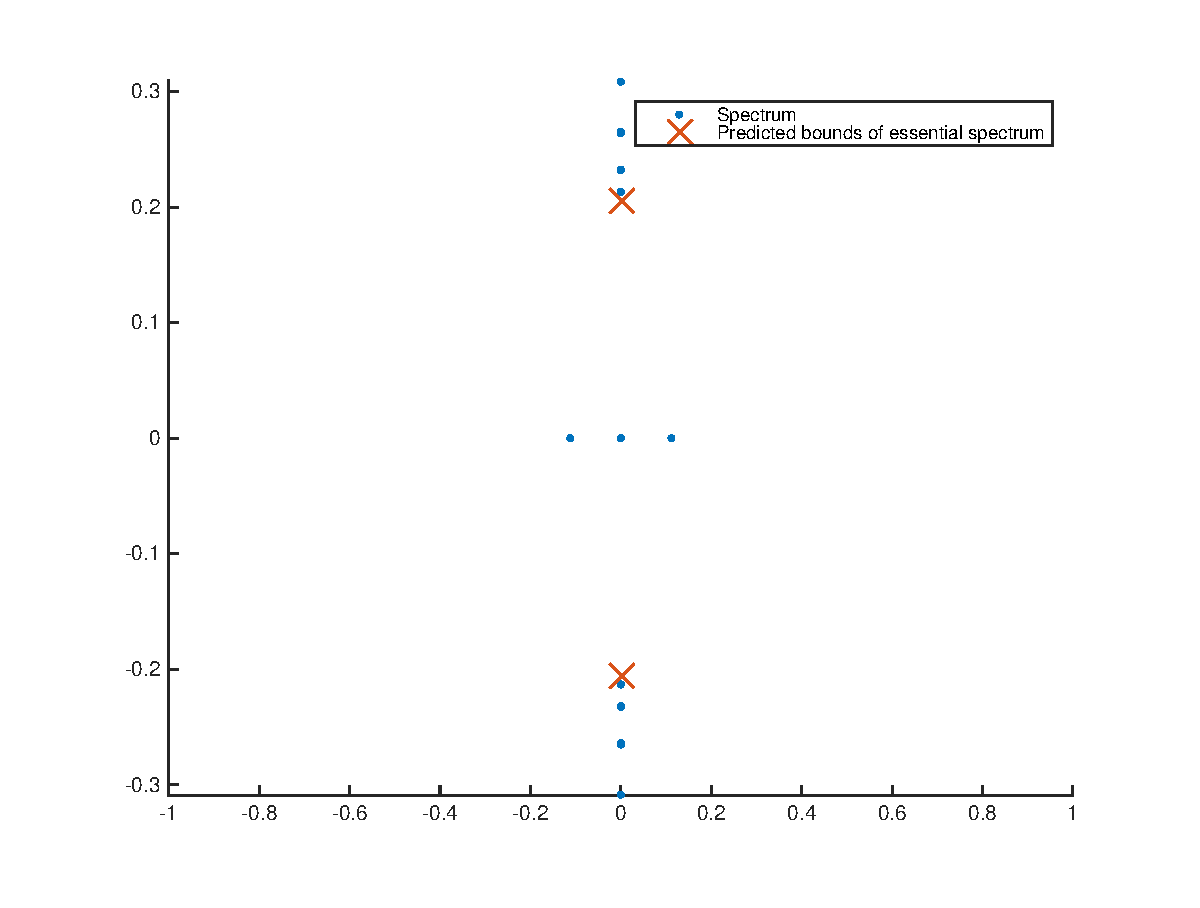
\includegraphics[width=8cm]{spec12_double1.eps}
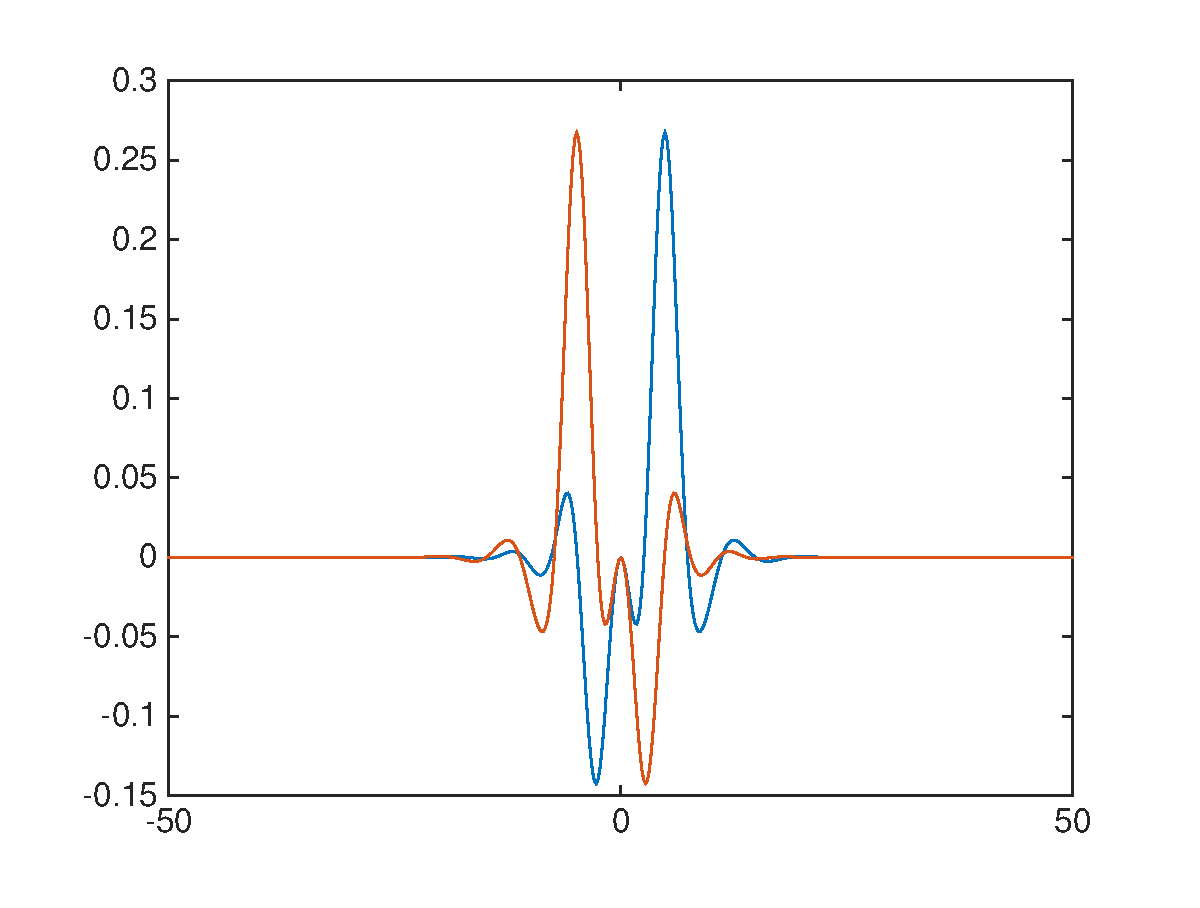
\includegraphics[width=8cm]{evecs12_double1.eps}
\caption{Linearization about Double Pulse 1. Spectrum (left) and interaction eigenfunctions (right). Finite difference methods, $N = 512$, $c = 1.2$.}
\end{figure}

Next we look at double pulse 2. Note that this time we have a pair of purely imaginary (to leading order; there is a small real part of order like 1e-10 just as with KdV5) eigenvalues. The plot below is only the real part of the eigenfunctions. It is easy to locate the interaction eigenvalues in this case, since we have bounds on the essential spectrum. The interaction eigenvalues lie inside the essential spectrum gap.

\begin{figure}[H]
\centering
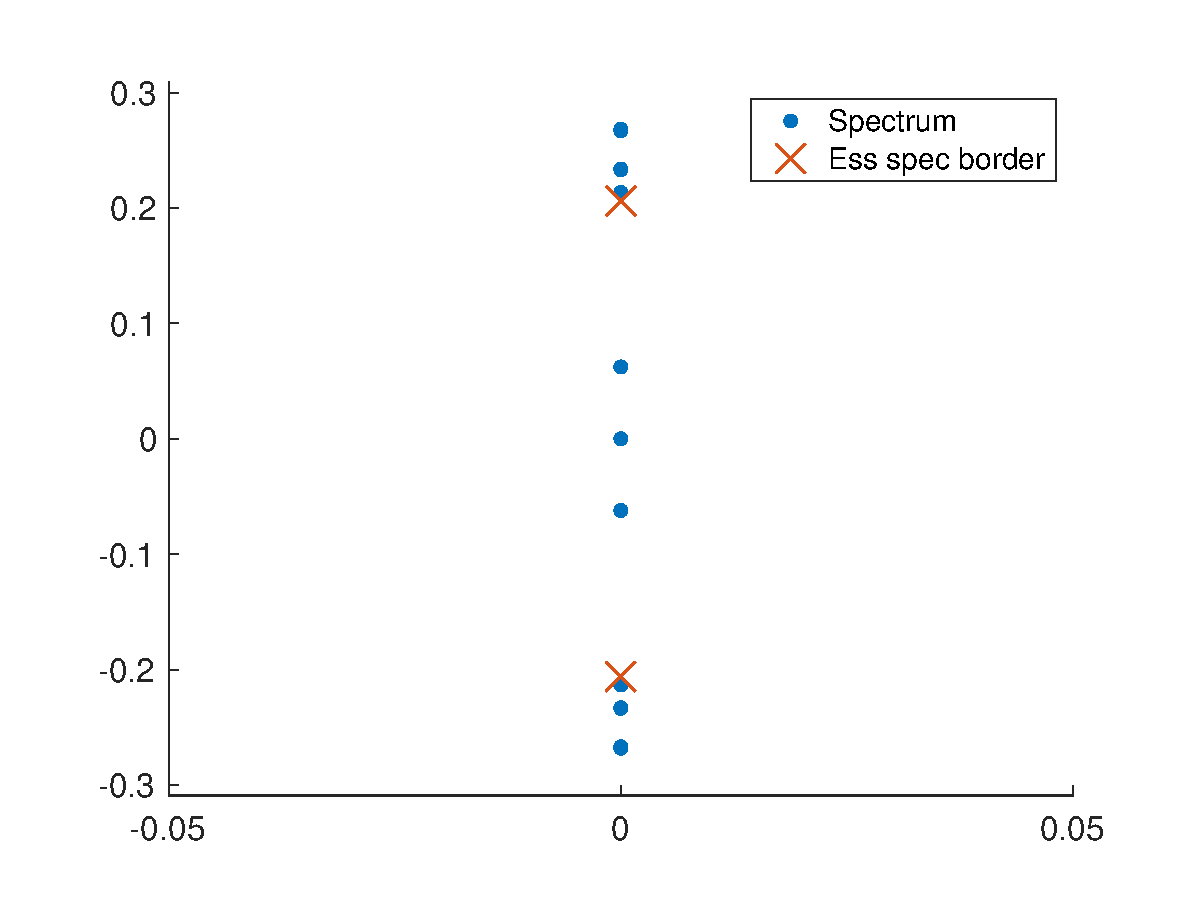
\includegraphics[width=8cm]{spec12_double2.eps}
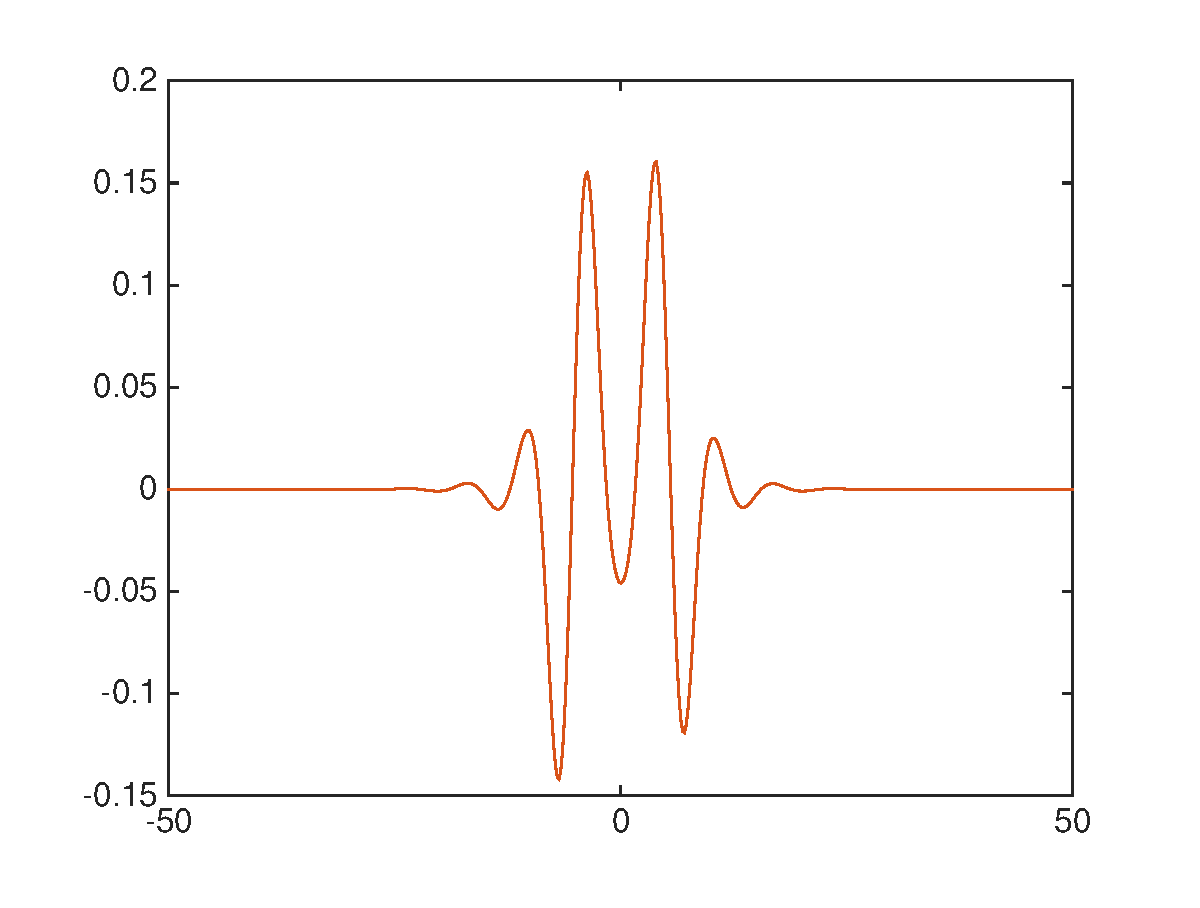
\includegraphics[width=8cm]{evecs12_double2real.eps}
\caption{Linearization about Double Pulse 2. Spectrum (left) and real part of interaction eigenfunctions (right). Finite difference methods, $N = 512$, $c = 1.2$.}
\end{figure}

The same pattern repeats (alternating pairs of real and purely imaginary interaction eigenvalues) as we go to higher double pulses.\\

We can also construct higher order multipulses. For example, here is a triple pulse for $c = 1.2$ using the same pulse distance as double pulse 2. We get the expected two pairs of purely imaginary eigenvalues.

\begin{figure}[H]
\centering
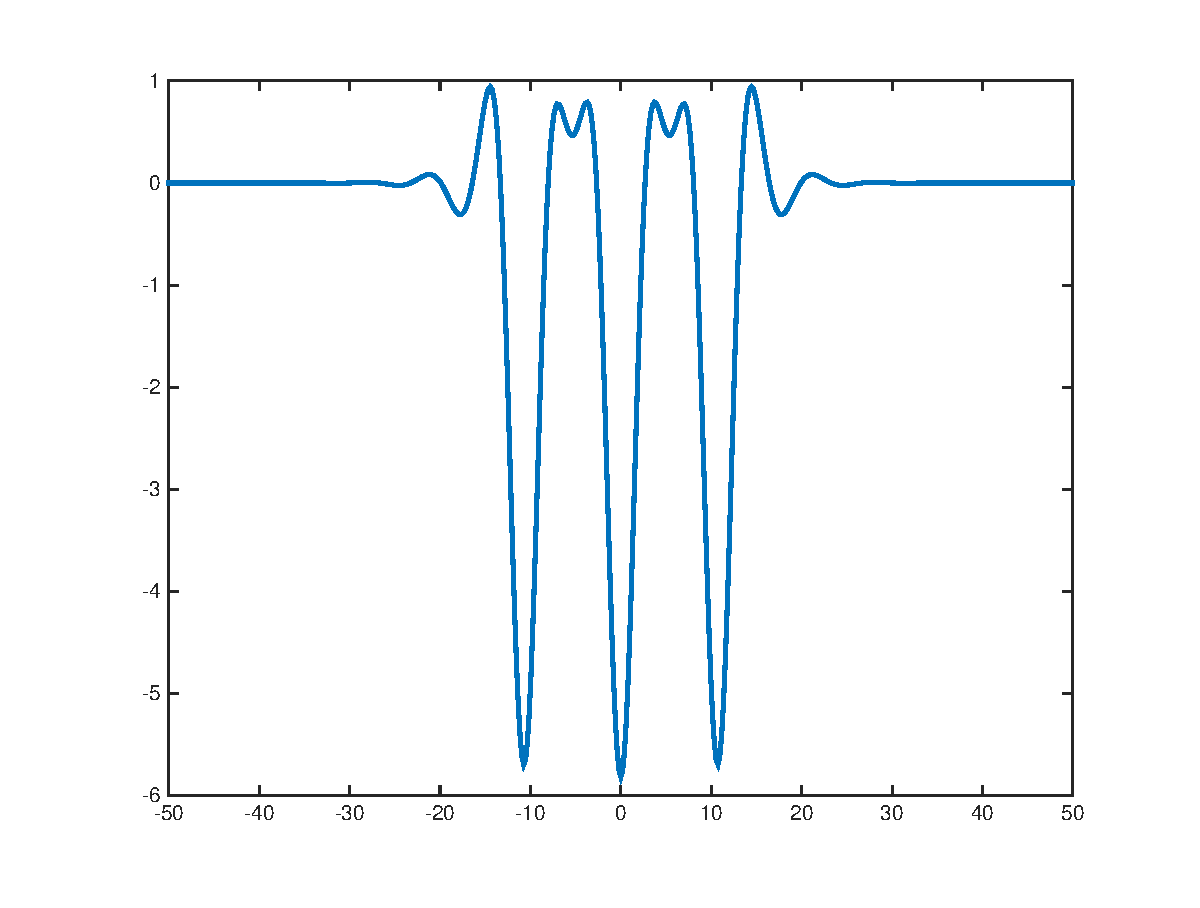
\includegraphics[width=8cm]{triple12_2.eps}
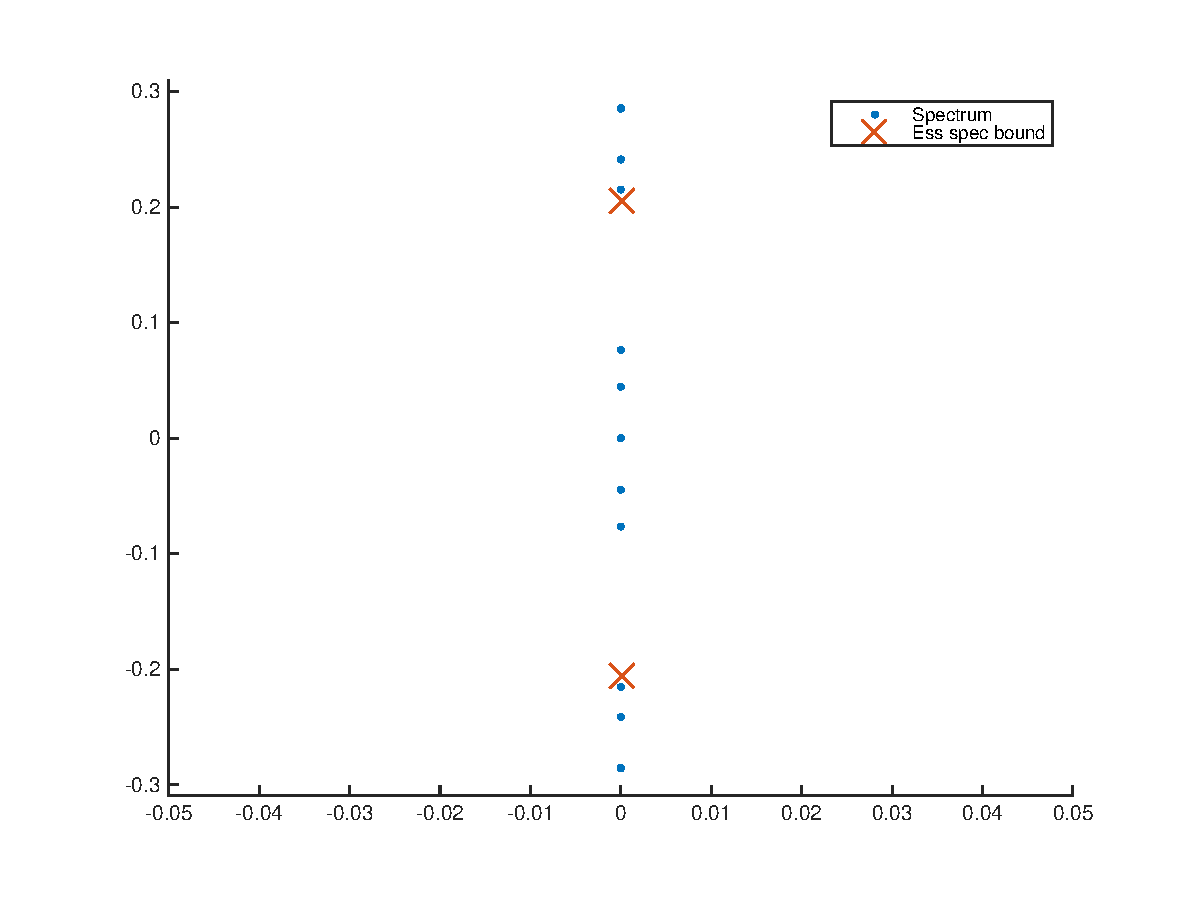
\includegraphics[width=8cm]{spec12_triple2.eps}
\caption{Triple pulse 2,2 (left). Spectrum of linearization about triple pulse 2,2 (right). Finite difference methods, $N = 512$, $c = 1.2$.}
\end{figure}

For other values of $c$, the odd-numbered double pulses have the same eigenvalue pattern, so we will focus on the even-numbered double pulses. Let's look at $c = 1.354$ (this value was used in \cite{Chen1997}). For Double Pulse 2, we now have a quartet of interaction eigenvalues. Their imaginary part now lies \emph{outside} the essential spectrum gap. This suggests that a Krein collision has occurred, where the interaction eigenvalues collide with the smallest essential spectrum eigenvalue and then form a quartet.

\begin{figure}[H]
\centering
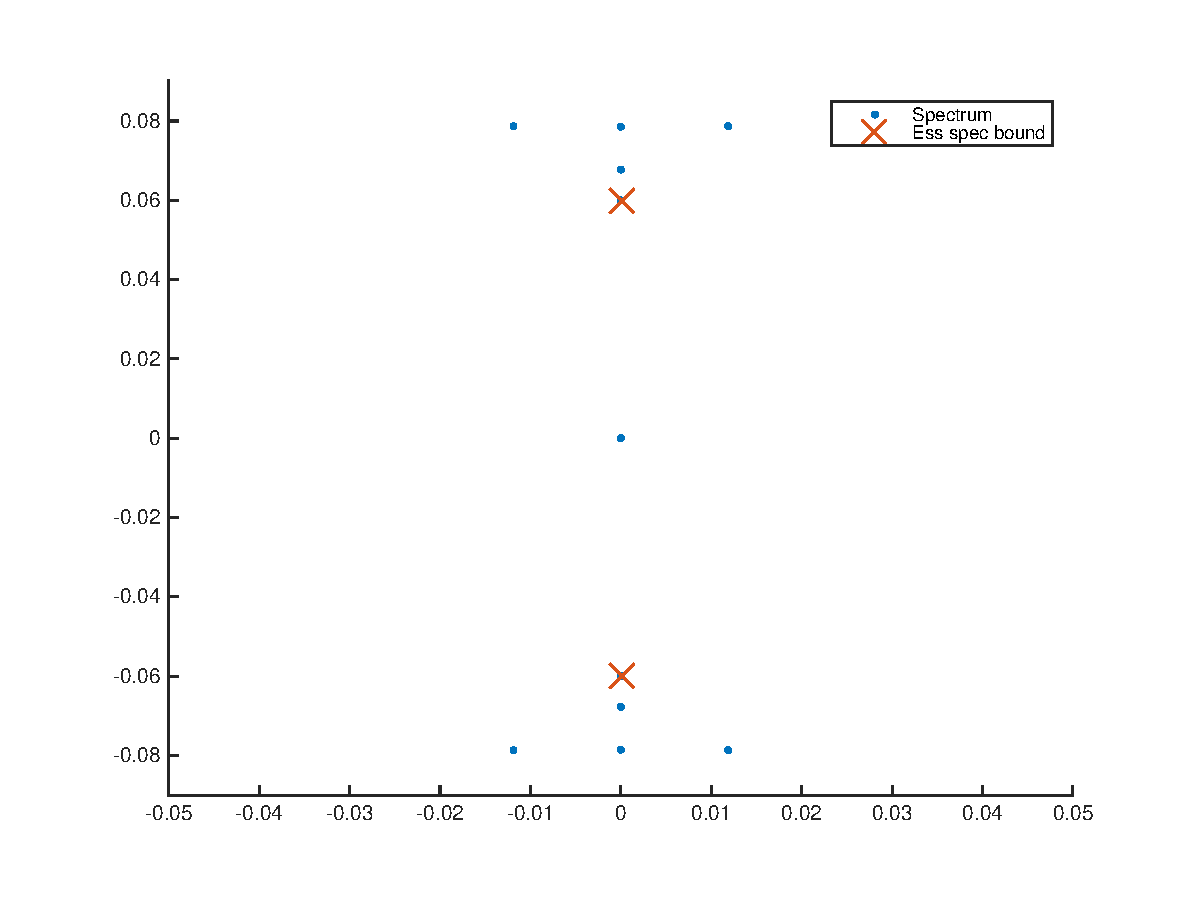
\includegraphics[width=8cm]{spec1354_double2.eps}
\caption{Linearization about Double Pulse 2. Spectrum showing Krein quartet. Finite difference methods, $N = 512$, $c = 1.354$.}
\end{figure}

The final two plots show that the Krein collision occurs between $c = 1.322$ (before collision) and $c = 1.323$ (after collision).

\begin{figure}[H]
\centering
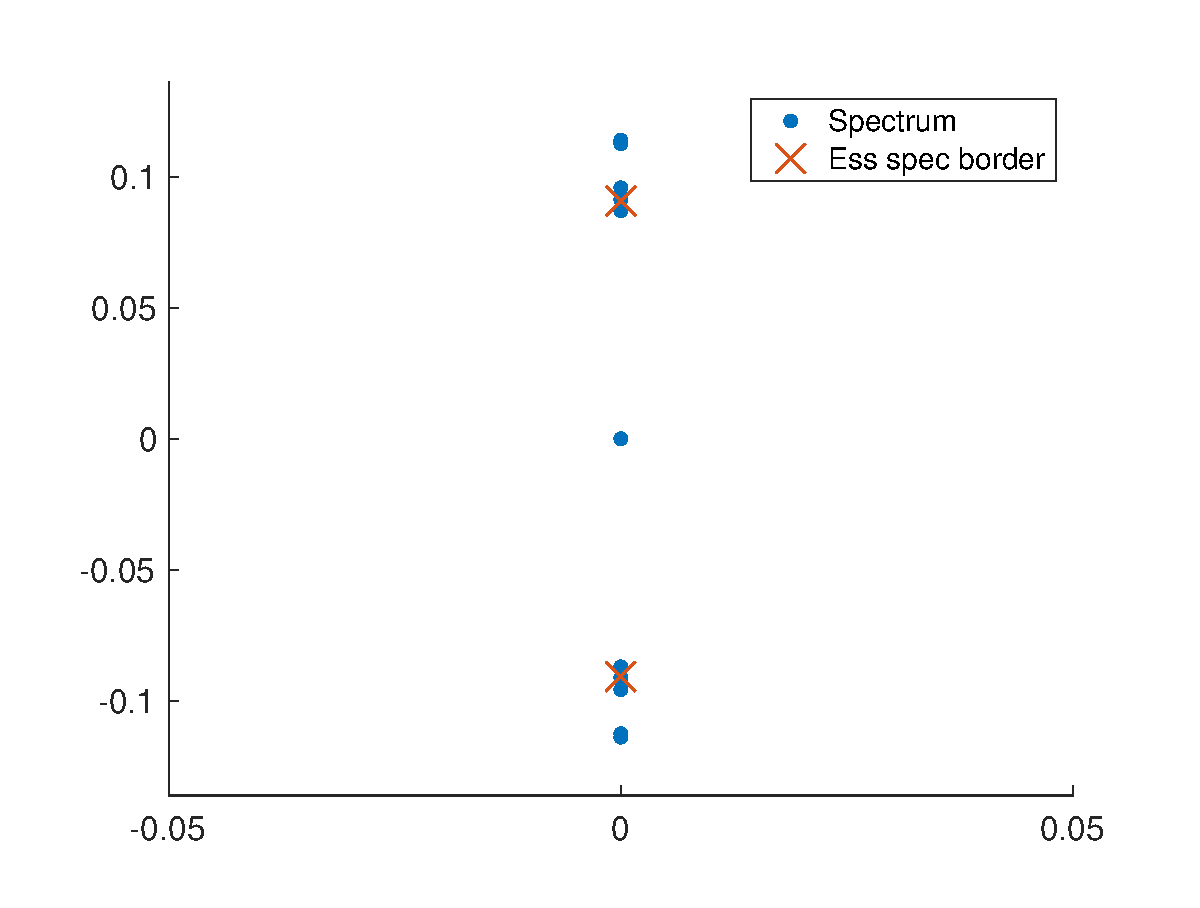
\includegraphics[width=8cm]{spec1322_double2.eps}
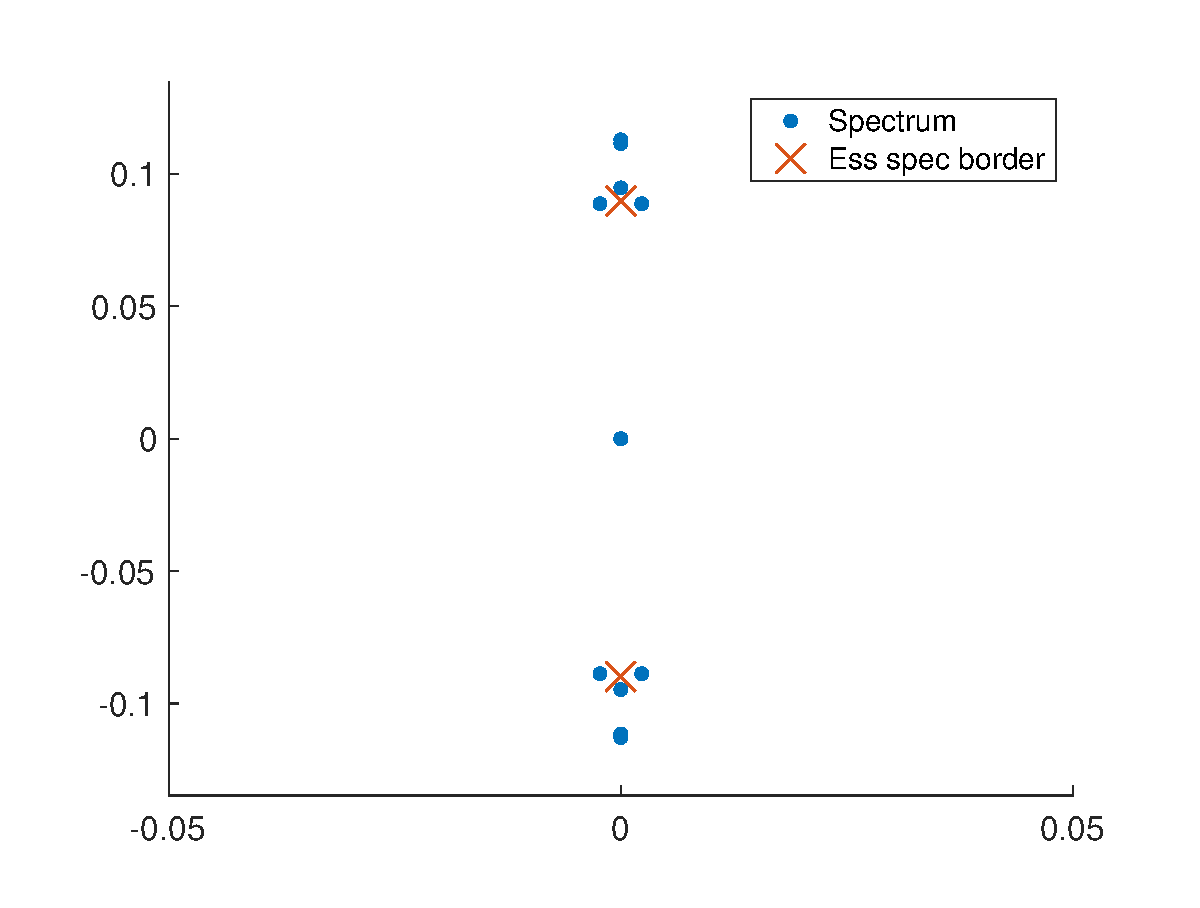
\includegraphics[width=8cm]{spec1323_double2.eps}
\caption{Linearization about Double Pulse 2. Spectrum before Krein collision ($c = 1.322$, left) and after Krein collision ($c = 1.323$, right). Finite difference methods, $N = 512$}
\end{figure}

\bibliography{suspension.bib}


\end{document}